\SetKwRepeat{Struct}{struct \{}{\}}%
\newcommand{\Array}{\KwSty{Array}}
\newcommand{\Integer}{\KwSty{Integer}}

\chapter{Task-Based, Parallel and Distributed Sparse Linear Algebra Applications \label{chap:exp_sparse}}
\graphicspath{{chapters/exp_sparse/}}

The sparse matrix vector product with several matrix storage format and matrix distribution across the computing resources is the basic algorithm considered in this chapter.
Sequences of sparse matrix products are important and largely used in several applications such as iterative methods and neural network training.
However, two executions of the sparse matrix vector are enough to outline the algorithmic issues without having to perform too much computations.
Therefore, the sparse operation $A(Ax+x)$ is considered as it uses two times the sparse matrix vector product.
We implement the sparse matrix vector algorithms previously introduced in Chapter \ref{chap:methods} with the selected task based programming models and perform numerical experiments on several clusters and supercomputers.
Finally, we discuss the results obtained in the experiments.


\section{Task-Based Methods for Parallel and Distributed Algorithms}
The sparse matrix vector product is executed in a distributed and parallel environment which means that computations can be run in parallel and data may not be accessed directly since they can be stored on a different resource than where they are needed.
The data can be moved through the network but it can be costly especially in very large networks.
The goal is to implement a parallel, distributed and task based sparse matrix vector product taking advantage of this set up while getting the best execution time and reducing the communications.
In the sparse matrix vector product case, the distributed and parallel algorithms (both regular and task based) depends on the storage formats used and the distribution of the sparse matrix on the distributed resources.
There is several way of distributing the matrix : either by splitting the columns or the rows.
A combination of the two previous way of distribution, the block distribution is also considered here.
They are the main way of distributing a matrix although other ways exist like a cyclic distribution where the consecutive values are put alternatively on a distributed resource.
The sub-matrices are stored in memory with a sparse storage format.


\subsection{Data Distribution \label{sec:sla:data_distribution}}

We consider three ways of distributing the data : a distribution by rows, by columns and by blocks.
The distribution by rows and by columns are special cases of the distribution by blocks where the is only distribution across one row for the distribution by columns and where the is only distribution across one column for the distribution by rows.
The blocks are sub-matrices kept on memory with a sparse storage format.
In this section, we are considering different ways of distributing sparse matrices.
However, we are not looking into the load balancing issues that may arise if some blocks are more populated than others.


\begin{figure}[h]
	\centering
	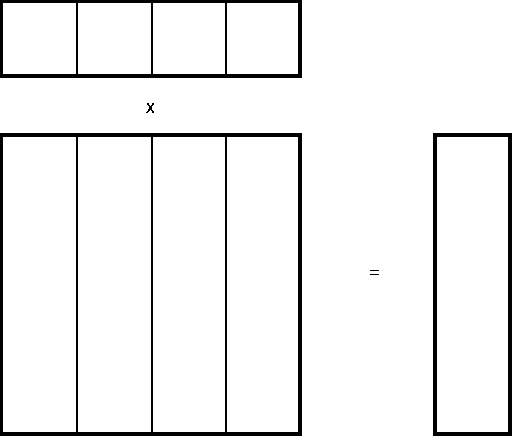
\includegraphics[width=.5\textwidth]{pmv_c}
	\caption{Distribution of the matrix by columns in which the sub-columns are compressed \label{fig:sparse:pmv_c}}
\end{figure}

The distribution by columns consists in splitting the rows and keeping the values of the same column in the same computing resource.
These columns are stored in a sparse storage format locally.
The input vector can also be split since only the rows of the vector corresponding to the columns stored in a computing resource are necessary for the matrix vector product.
The Figure \ref{fig:sparse:pmv_c} shows a matrix distributed by rows to make a matrix product vector as well as the necessary input vector and the result vector.
The result vector has the same size as the number of rows in the sub-matrices.
In this case, it corresponds to the full matrix number of rows.
However, each computing resource contains a part of the global solution of the matrix vector product.
To obtain the global result, all the distributed results have to be summed.


\begin{figure}[h]
	\centering
	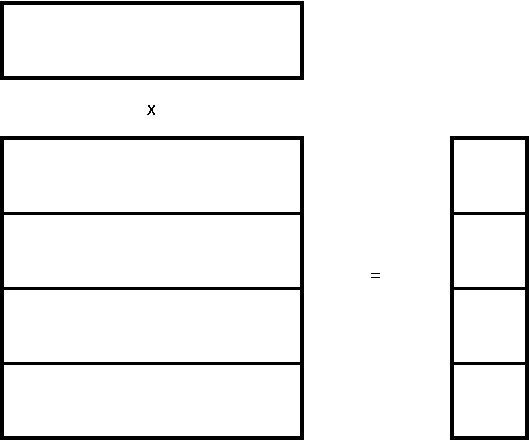
\includegraphics[width=.5\textwidth]{pmv_r}
	\caption{Distribution of the matrix by rows in which the sub-rows are compressed \label{fig:sparse:pmv_r}}
\end{figure}

The distribution by rows consists in splitting the columns and keeping the values of the same row in the same computing resource.
These rows are stored in a sparse storage format locally.
In this case, the input vector cannot be split since a complete row of the matrix may be stored in each computing resource.
In the sparse case, the rows may not be complete on each process but it can not be known in advance.
The input vector is duplicated in each computing resource.
The result vector has the same size as the number of rows in the sub-matrices.
Here, it corresponds to the number of rows in each corresponding sub-matrices.
However, each computing resource contains a sub-vector.
To obtain the global result, all the distributed results have to be gathered (which means that the global vector has just to be reconstructed without any computations).


\begin{figure}[h]
	\centering
	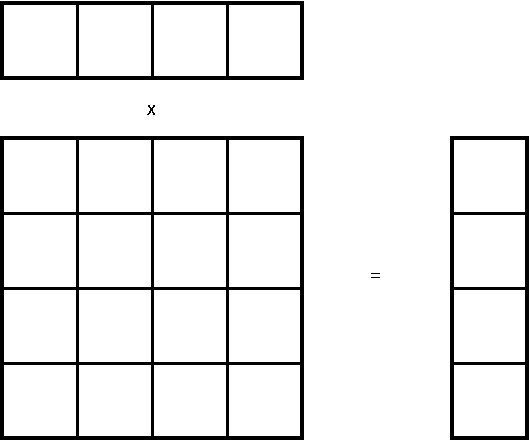
\includegraphics[width=.5\textwidth]{pmv_2D}
	\caption{Distribution of the matrix by rows and columns in which the blocks are compressed matrices \label{fig:sparse:pmv_2D}}
\end{figure}

The block distribution consists in both a distribution by rows and distribution by columns.
The matrix in split in a 2D grid way.
The $Nx \times Ny$ matrix is split in $Ngx \times Ngy$ sub-matrices.
The sub-matrices are stored in a sparse storage format locally.
In this case, the input vector is split across the columns of the matrix and the sub-vectors are duplicated on the sub-rows of the same column.
The Figure \ref{fig:sparse:pmv_r} shows a matrix distributed by blocks to perform a matrix product vector as well as the necessary input vector and the result vector with $Ngx = 4$ and $Ngy = 4$.
The result vector has the same size as the number of rows in the sub-matrices of the corresponding row.
However, each computing resource contains a part of a sub-vector.
To obtain the global result, all the distributed results of the same row have to be reduced then each rows have to be gathered if the full result vector is needed in one place.

The data distribution determines which part of the global matrix iq stored on a given computing resource.
The Section \ref{sec:sla:task_definition} points out how these data is used to perform the matrix vector product.

\subsection{Tasks Definition \label{sec:sla:task_definition}}

In this section, we consider that the matrix is divided according to one of the distribution described previously (except for the COO storage format).
Each sub-matrix is used as input of the matrix vector product tasks defined in the following algorithms.
We define data structures to store the matrices and use them in the tasks.
Finally, the algorithms for the tasks is designed.


\begin{algorithm}[h]
	\DontPrintSemicolon
	\SetAlgoVlined
	\caption{COO format data structure and matrix vector product\label{alg:sparse:spmv_coo}}
	\SetKwProg{Fn}{Task}{}{end}

	\Struct{MatrixCOO}{
		\Array{} row, col, val\;
	}
	\;
	\Fn{spmv\_coo()}{
		\KwData{m : MatrixCOO, v : Array}
		\KwResult{r : Array}
		\For{i \KwFrom 0 \KwTo m.val.size() - 1}{
			r[m.row[i]] += m.val[i] * v[m.col[i]]\;
		}
	}
\end{algorithm}

Algorithm \ref{alg:sparse:spmv_coo} defines a data structure to store the sub-matrices stored in the COO format.
It also shows the algorithm to make a matrix vector product on the sub-matrix given the proper input vector.
The data structure contains the three arrays necessary to store the matrix in the COO storage format.
In this implementation of the matrix vector product with the COO format, the sub-matrix does not have to be sorted e.g. this implementation does not expect the coordinates of the values of the matrix to be in a given range.
Therefore, this implementation can process any value in any position in any sub-matrix (which is not the case with the other storage formats).
However, we cannot deduce the range of position in the full input vector which is effectively used in the task as well as the range of position for the output vector since there is no restrictions on the range of coordinates of the values in the matrix.
Thus, this task also expect the full vector as input for the tasks (independently of the data distribution described) and output a full vector.

It can allow a better load balancing at the cost of a full vector in input and output which change how the output vector is processed to construct the full output vector.
This is discussed in Section \ref{sec:sla:task_based_parallel_algorithms}.


\begin{algorithm}[h]
	\DontPrintSemicolon
	\SetAlgoVlined
	\caption{SCOO format data structure and matrix vector product\label{alg:sparse:spmv_scoo}}
	\SetKwProg{Fn}{Task}{}{end}

	\Struct{MatrixSCOO}{
		\Array{} row, col, val\;
		\Integer{} fr, fc\;
	}
	\;
	\Fn{spmv\_scoo()}{
		\KwData{m : MatrixCOO, v : Array}
		\KwResult{r : Array}
		\For{i \KwFrom 0 \KwTo m.val.size() - 1}{
			r[m.row[i] - m.fr] += m.val[i] * v[m.col[i] - m.fc]\;
		}
	}
\end{algorithm}

Algorithm \ref{alg:sparse:spmv_scoo} defines a data structure to store the sub-matrices stored in the SCOO format in which we expect a given range of coordinates for the values contrary to the COO format.
It also shows the algorithm to make a matrix vector product on the sub-matrix given the proper input vector.
The data structure contains the three arrays necessary to store the matrix in the SCOO storage format as well as useful information about the position of the sub-matrix in the global matrix.
This information is the first row (\textit{fr}) and the first column (\textit{fc}) possibles in the sub-matrix (It may not correspond to the actual values stored in the sub-matrix since it corresponds to the lower boundaries of the possible coordinates in the sub-matrix for the algorithm to work properly).
The algorithm for the SCOO storage format is similar to the algorithm for COO whereas the supplementary information is used in the algorithm to properly position the output vector.
In this case, the range of position for the input and output vectors can be computed since the range of coordinates for the values in the SCOO storage format are restricted to the data distributions discussed in Section \ref{sec:sla:data_distribution}.
Therefore, depending of the data distribution, the input and output vector shapes change.

In this case, the construction of the full output vector depends on the division of the matrix as specified in Section \ref{sec:sla:data_distribution}.
This is detailed further in Section \ref{sec:sla:task_based_parallel_algorithms}.


\begin{algorithm}[h]
	\DontPrintSemicolon
	\SetAlgoVlined
	\caption{CSR format data structure and matrix vector product\label{alg:sparse:spmv_csr}}
	\SetKwProg{Fn}{Task}{}{end}

	\Struct{MatrixCSR}{
		\Array{} idx, col, val\;
		\Integer{} fc\;
	}
	\;
	\Fn{spmv\_csr()}{
		\KwData{m : MatrixCSR, v : Array}
		\KwResult{r : Array}
		\For{i \KwFrom 0 \KwTo m.idx.size() - 1}{
			\For{j \KwFrom m.idx[i] \KwTo m.idx[i+1] - 1}{
				r[i] += m.val[j] * v[m.col[j] - m.fc]\;
			}
		}
	}
\end{algorithm}

Algorithm \ref{alg:sparse:spmv_csr} defines a data structure to store the sub-matrices stored in the CSR format in which we expect a given range of coordinates for the values.
It also shows the algorithm to make a matrix vector product on the sub-matrix given the proper input vector.
The data structure contains the three arrays necessary to store the matrix in the CSR storage format as well as useful information about the position of the sub-matrix in the global matrix.
This information is the first column (\textit{fc}) possibles in the sub-matrix.
As for the SCOO storage format, the ranges of position for the input and output vectors can be computed.


\begin{algorithm}[h]
	\DontPrintSemicolon
	\SetAlgoVlined
	\caption{ELL format data structure and matrix vector product\label{alg:sparse:spmv_ell}}
	\SetKwProg{Fn}{Task}{}{end}

	\Struct{MatrixELL}{
		\Array{} col, val\;
		\Integer{} fc, max\_col\;
	}
	\;
	\Fn{spmv\_ell()}{
		\KwData{m : MatrixELL, v : Array}
		\KwResult{r : Array}
		\For{i \KwFrom 0 \KwTo m.lrs - 1}{
		 	\For{j \KwFrom 0 \KwTo m.max\_col - 1}{
		 		r[i + m.rpos] += m.val[i * m.max\_col + j] * v[m.col[i * m.max\_col + j]- m.fc]\;
		 	}
		}
	}
\end{algorithm}

Algorithm \ref{alg:sparse:spmv_ell} defines a data structure to store the sub-matrices stored in the ELL format in which we expect a given range of coordinates for the values.
It also shows the algorithm to make a matrix vector product on the sub-matrix given the proper input vector.
The data structure contains the number of columns needed in the arrays and the two arrays necessary to store the matrix in the ELL storage format as well the first column (\textit{fc}) possibles in the sub-matrix which is used in this algorithm.
As for the SCOO and CSR storage formats, the ranges of position for the input and output vectors can be computed.

In this section, we presented the algorithms used to perform the matrix vector product on the sub-matrices in the tasks with the COO, SCOO, ELL and CSR sparse storage formats.
They are used to perform the matrix vector product on the global matrix.
The Section \ref{sec:sla:task_based_parallel_algorithms} introduces the task-based algorithms to perform the sparse matrix vector product and construct the complete output vector.

\subsection{Task-Based Parallel Algorithms \label{sec:sla:task_based_parallel_algorithms}}

In this section, we introduce the task-based algorithms for the high level sparse matrix vector product.
They use the tasks designed in Section \ref{sec:sla:task_definition} to perform the matrix vector product on the global matrix.
In the algorithms the \textit{SPMV} tasks corresponds to one of the \textit{spmv\_*} defined in the previous section except for \textit{spmv\_coo} which needs a different data distribution.
These high level task-based algorithms are independent of the matrix storage format.


\begin{algorithm}[h]
	\DontPrintSemicolon
	\caption{Parallel and Distributed Task Based Algorithm for the Sparse  Matrix Vector Product with Distributed Rows \label{alg:sparse:task_spmv_rows}}
	\ParFor{i \KwFrom 0 \KwTo $Ngr - 1$}{
		M[i] = GenMatrix(i, $Ngr$, $Nr$, $Nc$)\;
	}
	V = GenVector($Ngc$)\;
	\;
	\ParFor{i \KwFrom 0 \KwTo $Ngr - 1$}{
		R[i] = SPMV(M[i], V)\;
	}
	\;
	\tcc{Necessary data migrations to relocate data for a new SPMV}
	\If{dataRelocation}{
		V = MERGE(R[0 : $Ngr - 1$])\;
	}

\end{algorithm}

Algorithm \ref{alg:sparse:task_spmv_rows} performs the matrix vector product on the global matrix when it is distributed by rows as shown in Figure \ref{fig:sparse:pmv_r}.
First, we need to generate or load the initial sub-matrices and sub-vectors to use them in the tasks.
With this data distribution, each task needs the full vector and output a piece of vector.
Then, the \textit{SPMV} tasks can be run on each sub-matrix.
Finally, the output vector has to be reconstructed.
In this case, we need to combine each of the output pieces of vector and create a full vector that can be reused later on.


\begin{algorithm}[h]
	\DontPrintSemicolon
	\caption{Parallel and Distributed General Task Based Algorithm for the Sparse  Matrix Vector Product with Distributed Columns \label{alg:sparse:task_spmv_col}}
	\ParFor{j \KwFrom 0 \KwTo $Ngc - 1$}{
		M[j] = GenMatrix(j, $Ngc$, $Nr$, $Nc$)\;
		V[j] = GenVector(j, $Ngc$, $Nc$)\;
	}
	\;
	\ParFor{j \KwFrom 0 \KwTo $Ngc - 1$}{
		Rl[j] = SPMV(M[j], V[j])\;
	}
	\;
	\tcc{Necessary data migrations to relocate data for a new SPMV}
	\uIf{dataRelocation}{
%		Rg = REDUCE(Rl[0 : $Ngc - 1$])\;
%		V[0 : $Ngc - 1$] = BROADCAST(Rg)\;
		\ParFor{j \KwFrom 0 \KwTo $Ngc - 1$}{
			V[j] = SUM(Rl[0 : $Ngc - 1$])\;
		}
	}
	\Else {
		Rg = SUM(Rl[0 : $Ngc - 1$])\;
	}
\end{algorithm}

Algorithm \ref{alg:sparse:task_spmv_col} performs the matrix vector product on the global matrix when it is distributed by columns as shown in Figure \ref{fig:sparse:pmv_c}.
With this data distribution, each task needs the only the piece of vector required to make the matrix vector product and output a full vector.
Then, the \textit{SPMV} tasks can be run on each sub-matrix.
In this case, the reconstruction of the full output vector is made by summing all the vectors which are results of the \textit{SPMV} task.


\begin{algorithm}[h]
	\DontPrintSemicolon
	\caption{Parallel and Distributed Task Based Algorithm for the Sparse  Matrix Vector Product with 2D Distributed Matrices \label{alg:sparse:task_spmv_2D}}
	\ParFor{j \KwFrom 0 \KwTo $Ngc - 1$}{
		\ParFor{i \KwFrom 0 \KwTo $Ngr - 1$}{
			M[i, j] = GenMatrix(i, j, $Ngr$, $Ngc$, $Nr$, $Nc$)\;
		}
		V[j] = GenVector(j, $Ngc$, $Nc$)\;
	}
	\;
	\ParFor{i \KwFrom 0 \KwTo $Ngr - 1$}{
		\ParFor{j \KwFrom 0 \KwTo $Ngc - 1$}{
			Rl[i, j] = SPMV(M[i, j], V[j])\;
		}
	}
	\ParFor{j \KwFrom 0 \KwTo $Ngc - 1$}{
		V[j] = SUM(Rl[i, 0 : $Ngc - 1$])\;
	}
	\;
	\If{dataRelocation}{
		Vm = MERGE(R[0 : $Ngr - 1$])\;
	}
\end{algorithm}

Algorithm \ref{alg:sparse:task_spmv_2D} performs the matrix vector product on the global matrix when it is distributed as shown in Figure \ref{fig:sparse:pmv_2D}.
With the 2D data distribution, each column of sub-matrices needs the corresponding sub-part of the input vector.
Then, the \textit{SPMV} tasks can be run on each sub-matrix.
In this case, the reconstruction of the full output vector is made by summing all the vectors which are results of the \textit{SPMV} task from the same row of sub-matrices then gathering the result of the sum in a complete vector.

\begin{algorithm}[h]
	\DontPrintSemicolon
	\caption{Parallel and Distributed Task Based Algorithm for the Sparse  Matrix Vector Product with COO matrices \label{alg:sparse:task_spmv_COO}}
	\ParFor{j \KwFrom 0 \KwTo $N - 1$}{
		M[i] = GenMatrixCOO(i, $N$, $Nr$, $Nc$)\;
	}
	V = GenVector($Nc$)\;
	\;
	\ParFor{j \KwFrom 0 \KwTo $Ngc - 1$}{
		Rl[i, j] = SPMV(M[i, j], V[j])\;
	}
	\;
	V = SUM(Rl[0 : $N - 1$])\;
\end{algorithm}

Algorithm \ref{alg:sparse:task_spmv_COO} performs the matrix vector product on the global matrix when it is distributed as a non restricted and split COO sparse storage format.
The matrix is split so that there is the same amount of values in each sub-matrix.
This improves the load balancing of the computations in the tasks (each task has the same number of computations).
With this data distribution, the shape of the input and output vectors cannot be anticipated so the matrix vector product task expect the full vector as input and return a full vector.
Then, to compute the output of the global matrix vector product, the output vector of each task has to be summed.

This section introduced the data distribution considered in this study.
They are a division by blocks of rows, blocks of columns, rectangle blocks in the rows and columns and a distribution with the same number of value in each task.
We also introduced the algorithms to implement the tasks for the sub-matrices with the different sparse matrix storage formats (COO, SCOO, ELL and CSR) as well as the task-based algorithms to perform the matrix vector product on the global matrix.
These algorithms are used to implement a task-based sparse matrix vector application and compare the performances obtained across different programming models, matrix storage format and data distribution in Section \ref{sec:sla:exp}.

\section{Numerical Experiments \label{sec:sla:exp}}
In this section, a sparse matrix vector product using task based, distributed and parallel programming models as well as the numerical experiments performed.
Three classes of programming models were chosen to implement the sparse matrix vector product.
First, MPI, a message passing library was chosen since it is the main stream library used to perform communications and global operation across multiple nodes on supercomputers.
Secondly, we chose to use a fine grain task based programming model in which dependencies between tasks are data oriented.
HPX, Legion and PaRSEC are such programming models and we chose to use only HPX since they cover the same kind of properties.
Finally, the last class is a parallel and distributed task based programming model in which tasks themselves are also parallel and distributed on a subset of the resources allocated to the application.
In this case, YML+XMP was chosen over Pegasus and Swift since YML+XMP has been more used than the other two.

\subsection{Application Description}
The sparse matrix vector product and the sparse $A(Ax+x)$ has been implemented with MPI, HPX, and YML+XMP.
The sparse operation $A(Ax+x)$ is the combination of two sparse matrix vector product $Ax$ with additional sum with the $x$ vector.
Therefore, a kernel performing the sparse $Ax$ has been implemented with the different storage format and is used as the base in MPI, HPX and YML+XMP to perform the sparse matrix vector product on the sub-matrices distributed on the computing resources.
This kernel is called in the HPX and YML+XMP tasks and the MPI processes to perform the sparse matrix vector product on the local data.
Then the programming model is used to make the appropriate data migrations in order to combine and form the output vector according to the algorithms introduced in Section \ref{sec:sla:task_based_parallel_algorithms}.

The kernel is designed to perform the sparse matrix vector product on the sub-matrices obtained from the split of the global matrix.
The input matrix can be split over a 2D grid with particular cases in which there is only one column (split only across rows) or only one row (split only across columns) as introduced in Section \ref{sec:sla:data_distribution}.
The $N_r \times N_c$ matrix is divided into an $N_{gr} \times N_{gc}$ grid.
This kernel is called in the MPI processes to perform the sparse matrix vector product on the local matrices.
In MPI, $N_{gr} \times N_{gc}$ is equal to the number of avail processes in the application.
This allow each process to manage its sub-matrix.
The kernel is also called in HPX tasks to perform the sparse matrix vector product on the sub-matrix managed into a tasks.
For HPX, there is no particular restrictions on $N_{gr}$ and $N_{gc}$ since there is no obligations to execute tasks on each worker process, even though, these workers could be idling due to the lack of tasks.
Finally, the kernel is also used in YML+XMP components (tasks) to perform the sparse matrix vector product in each processes allocated to each sparse matrix vector product task.
Afterwards, the output vector is combined inside the tasks then combined at the level of the graph of tasks.
Each YML task has an allocated number of processes.
Therefore, in order to make sure that each process works on a sub-matrix, the number of sub-matrices ($N_{tr} \times N_{tc}$) in the grid of sub-matrices in the tasks have to match the number of processes allocated to the tasks.
In our application, each task has the same number of processes allocated, which means that, in order to fill each processes of the tasks, the number of rows (resp. columns) in the division of the global matrix has to match the number of rows (resp. columns) in the division of the matrix in the tasks multiplied by the number of rows (resp. columns) in the division of the matrix at the task level (see Figure \ref{fig:sparse:yml_matrix_div}).

\begin{figure}[h]
        \centering
		\includegraphics[width=.4\textwidth]{{{yml_matrix_div}}}
        \caption{Two level of division in matrices managed by YML+XMP \label{fig:sparse:yml_matrix_div} with $3 \times 3$ task level matrices in which there is $4 \times 4$ sub-matrices}
\end{figure}

The kernel has been implemented to support the CSR, ELL, COO, SCOO and dense storage formats.
The sparse matrix vector products for the different storage formats were implemented according to the algorithms introduced in Section \ref{sec:sla:task_definition}.
Then, for each storage format and each programming model considered, the distributed and parallel version of the sparse matrix vector has been implemented based on the algorithms described in Section \ref{sec:sla:task_based_parallel_algorithms}.

Moreover, the sparse operation $A(Ax+x)$ has also been implemented on top the sparse matrix vector product.
Therefore, it also supports the CSR, ELL, COO, SCOO and dense storage formats as well as the different matrix distribution possibilities.
This operation has been implemented in MPI, HPX and YML+XMP.
It consists in a call to the sparse matrix vector product followed by the sum of the output vector with $x$ then another sparse matrix vector product.
The communications, the building of the output vector depending on the distribution of the matrix and the sum are managed with the programming models in which the application is implemented.

Finally, separate libraries containing the kernel as well as the MPI and HPX extensions of the kernel has been created.
YML+XMP does not support the creation of libraries therefore, the sparse matrix vector product and the sparse operation $A(Ax+x)$ were directly implemented as applications.
The libraries also contain functions to generate distributed sparse matrices and the YML+XMP applications has tasks for this purpose.
The sparse matrices can be generated in each one of the supported storage format and in the data distribution introduced in Section \ref{sec:sla:data_distribution}.
These matrices are the C-diagonal Q-perturbed matrices introduced in Chapter \ref{chap:methods}.
They are were used to perform numerical experiments which is presented in the next section.


\subsection{Results and Analyses on Total Petascale Pangea II}
In these experiments, the sparse operation $A(Ax+x)$ has been performed on a sparse matrix stored COO, SCOO, ELL and CSR where $A$ is the sparse matrix and $x$ a vector.
This operation has been chosen as test due to the fact that the output vector has to be recombined after the local sparse matrix vector in order to reuse it in the next sparse matrix vector product.
The C-diagonal Q-perturbed matrices introduced in Chapter \ref{chap:methods} are used to evaluate the performances of the different programming models and storage formats.
To do so, we perform strong scaling experiments on 2 000 000 $\times$ 2 000 000 and 4 000 000 $\times$ 4 000 000 C-diagonal Q-perturbed matrices for C = 300 and several values of Q.
Moreover, we also study the impact of the number of values by rows by trying multiple values of C.
Finally, we perform weak scaling experiments with the C-diagonal Q-perturbed matrices for C=300 by increasing the number of values in the matrix depending on the number of cores used to run the application.

\subsubsection{Pangea II}
Pangea II is the supercomputer on which the experiments have been performed.
It is owned by Total and located in Pau, France.
This supercomputer is composed of nodes built with 2 Xeon E5-2680v3 12C 2.5GHz processors for a total of 220 800 cores.
The nodes are connected with Infiniband FDR interconnects.
It performs at 5.283 PFlop/s for Linpack and 162.692 TFlop/s for HPCG.

\subsubsection{Best Results Selection}
These experiments depend on several parameters.
The programming model is the first of them.
There are also the parameters related to the test matrices used, C and Q as well as the size of the matrix.
Moreover, the data distribution which can be represented by the 2D grid used to divide the matrix adds two more parameters, $N_{gr}$ and $N_{gc}$.
Finally, YML+XMP also adds several parameters to tune the two levels of parallelism it offers.
These parameters are the number of processes allocated per task, the grid used to divide the matrix in the tasks and the higher level grid used to determine which part of the matrix is used in tasks.
Even if these parameters are related, which reduces the range of values to try, there is a large amount of possibilities to try.

Therefore, after running the applications, despite using only a subset of the possible cases to try, a large number of runs for the different parameters is produced.
Then, we have to select the case that produces the best execution time depending on which case we want to display.
For instance, if we want the best case for MPI for a given matrix size, storage format, C, Q and a 2 nodes, the results change depending on the data distribution.
Thus, we have to select which data distribution has made the best performances.
The application is run multiple time for a given data distribution so we take the median execution time as metric to compare the different data distributions.
Then, we chose the case that has the best median (usually the smallest since we want the fastest execution time).

\subsubsection{Strong scaling with a 2 000 000 $\times$ 2 000 000 sparse matrix}
Strong scaling experiments on the operation $A(Ax+x)$ have been performed with a 2 000 000 $\times$ 2 000 000 sparse C-diagonal Q-perturbed matrices for C = 300 and several values of Q.
The matrix was stored in 4 storage formats : CSR, COO, SCOO and ELL.
The applications were implemented in MPI, HPX and YML+XMP.
We use a dense vector with fixed values that is generated during the execution of the applications.

\begin{figure}[h]
        \centering
        \includegraphics[width=.45\textwidth]{{{fig_pangea2_nr2000000_lHPX_fCSR}}}
        \includegraphics[width=.45\textwidth]{{{fig_pangea2_nr2000000_lHPX_fELL}}}
        \includegraphics[width=.45\textwidth]{{{fig_pangea2_nr2000000_lHPX_fCOO}}}
        \includegraphics[width=.45\textwidth]{{{fig_pangea2_nr2000000_lHPX_fSCOO}}}

        \caption{Strong scaling considering HPX and several storage formats for a 2 000 000 $\times$ 2 000 000 matrix with C = 300 on Pangea II. Legend is (model, format, Q). \label{fig:sla:pangea2_nr2000000_lHPX}}
\end{figure}

Figure \ref{fig:sla:pangea2_nr2000000_lHPX} summarizes the results obtained from the experiments with HPX in which the operation $A(Ax+x)$ is applied on a 2 000 000 $\times$ 2 000 000 sparse C-diagonal Q-perturbed matrices for C = 300 and a vector.
This figure shows the execution time for the different sparse storage formats depending on the number of nodes (cores).
For CSR, ELL and SCOO, HPX has a very good strong scalability up to 4 nodes then the performance improvement gained from the increase in computing resources diminishes.
ELL and CSR have close performances on small number of nodes and CSR is better when the number of nodes increases.
They perform better than the COO and SCOO.
COO is the slowest within the HPX implementations.
This format is a bit different since the values of the matrix are not restricted to a 2D grid like the others.
Therefore, the output of each local sparse matrix vector product has to be summed to generate the complete output and this vector has the size of the rows of the full matrix since we do not restrict the positions of the values in the sub-matrices of this format.
Furthermore, this sum is a very costly reduction since it concerns all the sub-matrices and the reduced vector is very large.

% todo update with results
The best data distribution for SCOO, CSR and ELL is 3, 4 or 6 sub-columns until 8 nodes and it starts to increase to 8 or 12 for 16 nodes.
For COO, there is no data distribution according to row or columns since it is divided according to a number of division.
In practice, the COO are divided in $N_{gr} \times N_{gc}$ where $N_{gr} \times N_{gc}$ is the grid in which the other storage format divide their matrix.
The best data distribution is similar for SCOO, CSR and ELL since they use the same pattern to combine the output vector.


\begin{figure}[h]
        \centering
        \includegraphics[width=.45\textwidth]{{{fig_pangea2_nr2000000_lMPI_fCSR}}}
        \includegraphics[width=.45\textwidth]{{{fig_pangea2_nr2000000_lMPI_fELL}}}
        \includegraphics[width=.45\textwidth]{{{fig_pangea2_nr2000000_lMPI_fCOO}}}
        \includegraphics[width=.45\textwidth]{{{fig_pangea2_nr2000000_lMPI_fSCOO}}}

        \caption{Strong scaling considering MPI and several storage formats for a 2 000 000 $\times$ 2 000 000 matrix with C = 300 on Pangea II. Legend is (model, format, Q). \label{fig:sla:pangea2_nr2000000_lMPI}}
\end{figure}

Figure \ref{fig:sla:pangea2_nr2000000_lMPI} summarizes the results obtained from the experiments with MPI in which the operation $A(Ax+x)$ is applied on a 2 000 000 $\times$ 2 000 000 sparse C-diagonal Q-perturbed matrices for C = 300 and a vector.
This figure shows the execution time for the different sparse storage formats depending on the number of nodes (cores).
CSR obtains the vest performances with MPI.
CSR and ELL have very close performances for Q = 0 and, for the other values of Q, it is SCOO who is very close to CSR.
CSR and SCOO perform better than ELL and COO.
COO is the slowest due to the fact that the output of each sub-matrix has to be summed and the output vector is of the size the global number of rows of the matrix.
However it is very close to ELL when Q > 0 despite its costly global reduction.

% todo update with results
The best data distribution for SCOO and CSR is 1 sub-row until 8 nodes.
Then, starting at 16 nodes, there is cases in which the best performances are with 1 sub-column.
For ELL, the best data distribution is with 1 sub-column except for 8 nodes where it is 4 sub-columns sometimes.
As with HPX, for COO, there is no data distribution according to row or columns.
It is interesting to notice that, SCOO and CSR obtain the best performances with the same data distribution and ELL best performances are obtained with another data distribution with MPI.


\begin{figure}[h]
        \centering
        \includegraphics[width=.45\textwidth]{{{fig_pangea2_nr2000000_lYML_fCSR}}}
        \includegraphics[width=.45\textwidth]{{{fig_pangea2_nr2000000_lYML_fELL}}}
        \includegraphics[width=.45\textwidth]{{{fig_pangea2_nr2000000_lYML_fCOO}}}
        \includegraphics[width=.45\textwidth]{{{fig_pangea2_nr2000000_lYML_fSCOO}}}

        \caption{Strong scaling considering YML and several storage formats for a 2 000 000 $\times$ 2 000 000 matrix with C = 300 on Pangea II. Legend is (model, format, Q).  \label{fig:sla:pangea2_nr2000000_lYML}}
\end{figure}

Figure \ref{fig:sla:pangea2_nr2000000_lYML} summarizes the results obtained from the experiments with YML in which the operation $A(Ax+x)$ is applied on a 2 000 000 $\times$ 2 000 000 sparse C-diagonal Q-perturbed matrices for C = 300 and a vector.
This figure shows the execution time for the different sparse storage formats depending on the number of nodes (cores).
% todo update with results
In COO and SCOO, the performances are quite stable and we obtain execution time close for the different values of Q.
Until 4 nodes, there is a slight improvement of performances  for COO and SCOO execution times stay almost constant.
Then, for the increase from 4 nodes to 8 nodes, the performances plummet dramatically.
We think it is due to the increasing number of processes making IOs (96 to 192) to communicate the data between the tasks since YML uses the file system to pass data.
This induces a great variability between the results.
On the other hand, CSR and ELL performances have more variability and it is difficult to find a logical pattern.
CSR seems to have better performances overall but there is some cases where the other storage formats are prevalent.

Furthermore, YML+XMP introduces more parameters to describe the data distribution in the tasks and across the different tasks.
This is an open set of parameters as the matrix can be divided into any shape.
Even though there is relation between the parameters, it is still a large amount of parameters to try out.
Moreover, due to technical issues, multiple YML+XMP applications cannot be run at same time while it is perfectly possible to run several MPI or HPX applications at the same time.
This greatly limit the range of parameters that can be tested since it is not possible to take advantage of the large amount of computing resources available.
The constraint to run only one application at a time and having a lot more parameters to try with YML+XMP lets the possibility of the existence of parameters that could produce better performances than the ones used in the current experiments.
We tried as much parameters we believed would lead to interesting results as we could.

%\begin{figure}[h]
%        \centering
%        \includegraphics[width=.45\textwidth]{{{fig_pangea2_nr2000000_lYML1x1_fCSR}}}
%        \includegraphics[width=.45\textwidth]{{{fig_pangea2_nr2000000_lYML1x1_fELL}}}
%        \includegraphics[width=.45\textwidth]{{{fig_pangea2_nr2000000_lYML1x1_fCOO}}}
%        \includegraphics[width=.45\textwidth]{{{fig_pangea2_nr2000000_lYML1x1_fSCOO}}}
%
%        \caption{Strong scaling considering YML with the matrix in only one block and several storage format for a 2 000 000 $\times$ 2 000 000 matrix with C = 300 on Pangea II. Legend is (model, format, Q). \label{fig:sla:pangea2_nr2000000_lYML1x1}}
%\end{figure}
%Figure \ref{fig:sla:pangea2_nr2000000_lYML1x1}
%\begin{table}[h]
%	\begin{tabular}{cccccccccccc}
\hline
Cases & Nodes& BGC& BGR& CPT& GC& GR& LGC& LGR& median & N & Ncase \\
\hline
\multirow{4}{*}{('YML', 'CSR', 0.0)}& 1& 1& 2& 24& 2& 24& 2& 12& 3.4773& 3& 16\\
& 2& 1& 2& 24& 24& 2& 24& 1& 3.0802& 5& 14\\
& 4& 2& 2& 48& 6& 32& 3& 16& 5.5149& 1& 20\\
& 8& 1& 2& 192& 1& 384& 1& 192& 5.4662& 5& 19\\
\hline
\multirow{4}{*}{('YML', 'CSR', 0.2)}& 1& 1& 2& 24& 1& 48& 1& 24& 3.1105& 3& 16\\
& 2& 2& 1& 48& 48& 2& 24& 2& 3.2017& 2& 14\\
& 4& 2& 2& 48& 6& 32& 3& 16& 5.593& 1& 20\\
& 8& 1& 2& 192& 1& 384& 1& 192& 5.7279& 5& 19\\
\hline
\multirow{4}{*}{('YML', 'CSR', 0.4)}& 1& 1& 2& 24& 2& 24& 2& 12& 3.2923& 3& 16\\
& 2& 1& 2& 24& 24& 2& 24& 1& 2.8888& 5& 14\\
& 4& 2& 1& 48& 96& 1& 48& 1& 3.5201& 2& 20\\
& 8& 1& 2& 192& 12& 32& 12& 16& 4.315& 3& 17\\
\hline
\multirow{4}{*}{('YML', 'CSR', 0.6)}& 1& 1& 2& 24& 2& 24& 2& 12& 3.3289& 3& 16\\
& 2& 1& 2& 24& 24& 2& 24& 1& 3.1826& 5& 14\\
& 4& 2& 1& 48& 96& 1& 48& 1& 3.9313& 2& 20\\
& 8& 1& 2& 192& 12& 32& 12& 16& 4.2311& 3& 17\\
\hline
\multirow{4}{*}{('YML', 'CSR', 0.8)}& 1& 1& 2& 24& 1& 48& 1& 24& 3.1635& 3& 16\\
& 2& 2& 1& 48& 48& 2& 24& 2& 3.0951& 2& 14\\
& 4& 2& 1& 48& 96& 1& 48& 1& 3.4505& 2& 20\\
& 8& 1& 2& 192& 12& 32& 12& 16& 4.1401& 3& 17\\
\hline
\multirow{4}{*}{('YML', 'CSR', 1.0)}& 1& 1& 2& 24& 2& 24& 2& 12& 3.0996& 3& 16\\
& 2& 2& 1& 48& 48& 2& 24& 2& 3.5524& 2& 14\\
& 4& 2& 1& 48& 96& 1& 48& 1& 4.1899& 2& 20\\
& 8& 1& 2& 192& 12& 32& 12& 16& 4.4705& 3& 18\\
\hline
\end{tabular}

%\end{table}
%\begin{table}[h]
%	\begin{tabular}{cccccccccccc}
\hline
Cases & Nodes& BGC& BGR& CPT& GC& GR& LGC& LGR& median & N & Ncase \\
\hline
\multirow{4}{*}{('YML', 'ELL', 0.0)}& 1& 1& 2& 24& 4& 12& 4& 6& 3.6421& 1& 10\\
& 2& 2& 1& 48& 4& 24& 2& 24& 4.0547& 3& 4\\
& 4& 2& 1& 48& 2& 48& 1& 48& 3.942& 7& 5\\
& 8& 1& 2& 192& 1& 384& 1& 192& 5.0715& 3& 6\\
\hline
\multirow{4}{*}{('YML', 'ELL', 0.2)}& 1& 1& 2& 24& 3& 16& 3& 8& 3.7532& 3& 10\\
& 2& 2& 1& 48& 4& 24& 2& 24& 6.6783& 2& 4\\
& 4& 2& 1& 48& 2& 48& 1& 48& 3.9821& 5& 5\\
& 8& 1& 2& 192& 1& 384& 1& 192& 7.1898& 3& 6\\
\hline
\multirow{4}{*}{('YML', 'ELL', 0.4)}& 1& 1& 2& 24& 3& 16& 3& 8& 3.924& 3& 10\\
& 2& 2& 1& 48& 4& 24& 2& 24& 4.3442& 3& 4\\
& 4& 2& 1& 48& 2& 48& 1& 48& 3.4307& 5& 5\\
& 8& 1& 2& 192& 1& 384& 1& 192& 6.7696& 3& 6\\
\hline
\multirow{4}{*}{('YML', 'ELL', 0.6)}& 1& 1& 2& 24& 2& 24& 2& 12& 3.7269& 3& 10\\
& 2& 2& 1& 48& 4& 24& 2& 24& 4.5151& 3& 4\\
& 4& 2& 1& 48& 2& 48& 1& 48& 4.1574& 5& 5\\
& 8& 1& 2& 192& 1& 384& 1& 192& 6.1698& 3& 6\\
\hline
\multirow{4}{*}{('YML', 'ELL', 0.8)}& 1& 1& 2& 24& 1& 48& 1& 24& 3.6055& 3& 9\\
& 2& 2& 1& 48& 4& 24& 2& 24& 5.4453& 3& 4\\
& 4& 2& 1& 48& 2& 48& 1& 48& 3.8436& 5& 5\\
& 8& 4& 1& 48& 16& 12& 4& 12& 9.3383& 1& 6\\
\hline
\multirow{4}{*}{('YML', 'ELL', 1.0)}& 1& 1& 2& 24& 2& 24& 2& 12& 4.002& 3& 9\\
& 2& 2& 1& 48& 4& 24& 2& 24& 4.1681& 3& 4\\
& 4& 2& 1& 48& 2& 48& 1& 48& 4.1922& 5& 5\\
& 8& 1& 2& 192& 1& 384& 1& 192& 6.8561& 3& 6\\
\hline
\end{tabular}


%python create_figure.py pangea2_tbsla_YML1x1.json -f op:a_axpx -f success:true -f matrixtype:cqmat -f machine:Pangea2 -l lang:YML -l format:ELL -l Q -l NR:2000000 -l C:300 -s GR -s GC -s LGR -s LGC -s BGR -s BGC -s CPT -coi nodes -voi time_op -o /Users/administrateur/Desktop/work/Thesis/phd_dissertation/chapters/exp_sparse/fig_pangea2_nr2000000_lYML_fELL.pdf -xlabel "Nodes (Cores)" -ylabel "Time (s)" -cpn 24


%\end{table}
%\begin{table}[h]
%	\begin{tabular}{cccccccccccc}
\hline
Cases & Nodes& BGC& BGR& CPT& GC& GR& LGC& LGR& median & N & Ncase \\
\hline
\multirow{4}{*}{('YML', 'COO', 0.0)}& 1& 1& 2& 24& 3& 16& 3& 8& 3.9307& 1& 16\\
& 2& 1& 2& 48& 2& 48& 2& 24& 3.5267& 1& 14\\
& 4& 2& 1& 48& 24& 4& 12& 4& 3.1323& 3& 16\\
& 8& 1& 2& 96& 2& 96& 2& 48& 5.394& 3& 14\\
\hline
\multirow{4}{*}{('YML', 'COO', 0.2)}& 1& 1& 2& 24& 6& 8& 6& 4& 3.849& 1& 16\\
& 2& 1& 2& 48& 2& 48& 2& 24& 3.0919& 1& 14\\
& 4& 2& 1& 48& 24& 4& 12& 4& 2.9645& 3& 17\\
& 8& 1& 2& 96& 2& 96& 2& 48& 6.3038& 3& 13\\
\hline
\multirow{4}{*}{('YML', 'COO', 0.4)}& 1& 1& 2& 24& 6& 8& 6& 4& 3.7139& 1& 15\\
& 2& 1& 2& 24& 24& 2& 24& 1& 3.1377& 3& 14\\
& 4& 1& 2& 96& 6& 32& 6& 16& 3.0372& 1& 17\\
& 8& 1& 2& 96& 1& 192& 1& 96& 5.9068& 3& 14\\
\hline
\multirow{4}{*}{('YML', 'COO', 0.6)}& 1& 1& 2& 24& 6& 8& 6& 4& 3.9468& 1& 15\\
& 2& 1& 2& 48& 2& 48& 2& 24& 3.2917& 1& 14\\
& 4& 2& 1& 48& 24& 4& 12& 4& 3.1861& 3& 17\\
& 8& 1& 2& 96& 1& 192& 1& 96& 5.6193& 3& 14\\
\hline
\multirow{4}{*}{('YML', 'COO', 0.8)}& 1& 1& 2& 24& 3& 16& 3& 8& 3.8611& 1& 15\\
& 2& 1& 2& 24& 24& 2& 24& 1& 3.1965& 3& 14\\
& 4& 2& 1& 48& 24& 4& 12& 4& 3.2131& 3& 17\\
& 8& 4& 1& 48& 12& 16& 3& 16& 6.9458& 2& 15\\
\hline
\multirow{4}{*}{('YML', 'COO', 1.0)}& 1& 1& 2& 24& 1& 48& 1& 24& 3.7985& 1& 16\\
& 2& 1& 2& 48& 2& 48& 2& 24& 3.4788& 1& 14\\
& 4& 2& 1& 48& 6& 16& 3& 16& 2.9228& 3& 17\\
& 8& 1& 2& 96& 1& 192& 1& 96& 6.4428& 3& 15\\
\hline
\end{tabular}


%python create_figure.py pangea2_tbsla_YML1x1.json -f op:a_axpx -f success:true -f matrixtype:cqmat -f machine:Pangea2 -l lang:YML -l format:COO -l Q -l NR:2000000 -l C:300 -s GR -s GC -s LGR -s LGC -s BGR -s BGC -s CPT -coi nodes -voi time_op -o /Users/administrateur/Desktop/work/Thesis/phd_dissertation/chapters/exp_sparse/fig_pangea2_nr2000000_lYML_fCOO.pdf -xlabel "Nodes (Cores)" -ylabel "Time (s)" -cpn 24


%\end{table}
%\begin{table}[h]
%	\begin{tabular}{cccccccccccc}
\hline
Cases & Nodes& BGC& BGR& CPT& GC& GR& LGC& LGR& median & N & Ncase \\
\hline
\multirow{5}{*}{('YML', 'SCOO', 0.0)}& 1& 1& 2& 24& 1& 48& 1& 24& 3.9036& 3& 16\\
& 2& 1& 2& 48& 2& 48& 2& 24& 3.4013& 1& 16\\
& 4& 2& 1& 48& 96& 1& 48& 1& 2.8016& 3& 17\\
& 8& 4& 1& 48& 12& 16& 3& 16& 8.7345& 2& 20\\
& 16& None& None& None& None& None& None& None& None& 0& 0\\
\hline
\multirow{5}{*}{('YML', 'SCOO', 0.2)}& 1& 1& 2& 24& 1& 48& 1& 24& 4.0968& 3& 16\\
& 2& 2& 1& 48& 4& 24& 2& 24& 3.2149& 1& 16\\
& 4& 2& 1& 48& 96& 1& 48& 1& 3.6747& 3& 18\\
& 8& 4& 1& 48& 12& 16& 3& 16& 8.1702& 2& 19\\
& 16& None& None& None& None& None& None& None& None& 0& 0\\
\hline
\multirow{5}{*}{('YML', 'SCOO', 0.4)}& 1& 1& 2& 24& 1& 48& 1& 24& 3.815& 3& 16\\
& 2& 1& 2& 24& 24& 2& 24& 1& 3.0734& 3& 16\\
& 4& 2& 1& 48& 96& 1& 48& 1& 3.4709& 3& 18\\
& 8& 4& 1& 48& 12& 16& 3& 16& 8.5992& 2& 20\\
& 16& None& None& None& None& None& None& None& None& 0& 0\\
\hline
\multirow{5}{*}{('YML', 'SCOO', 0.6)}& 1& 2& 1& 24& 48& 1& 24& 1& 3.7989& 1& 16\\
& 2& 1& 2& 48& 24& 4& 24& 2& 3.2484& 1& 17\\
& 4& 2& 1& 48& 96& 1& 48& 1& 3.5548& 3& 17\\
& 8& 4& 2& 48& 16& 24& 4& 12& 9.293& 1& 18\\
& 16& None& None& None& None& None& None& None& None& 0& 0\\
\hline
\multirow{5}{*}{('YML', 'SCOO', 0.8)}& 1& 1& 2& 24& 1& 48& 1& 24& 3.7747& 3& 16\\
& 2& 2& 1& 48& 48& 2& 24& 2& 3.2922& 1& 17\\
& 4& 2& 1& 48& 96& 1& 48& 1& 3.6671& 3& 17\\
& 8& 4& 1& 48& 16& 12& 4& 12& 8.5238& 1& 20\\
& 16& None& None& None& None& None& None& None& None& 0& 0\\
\hline
\multirow{5}{*}{('YML', 'SCOO', 1.0)}& 1& 1& 2& 24& 1& 48& 1& 24& 3.7833& 3& 16\\
& 2& 2& 1& 48& 48& 2& 24& 2& 3.2836& 1& 17\\
& 4& 2& 1& 48& 96& 1& 48& 1& 3.4435& 3& 18\\
& 8& 4& 1& 48& 16& 12& 4& 12& 8.7987& 1& 20\\
& 16& None& None& None& None& None& None& None& None& 0& 0\\
\hline
\end{tabular}


%python create_figure.py pangea2_tbsla_YML1x1.json -f op:a_axpx -f success:true -f matrixtype:cqmat -f machine:Pangea2 -l lang:YML -l format:SCOO -l Q -l NR:2000000 -l C:300 -s GR -s GC -s LGR -s LGC -s BGR -s BGC -s CPT -coi nodes -voi time_op -o /Users/administrateur/Desktop/work/Thesis/phd_dissertation/chapters/exp_sparse/fig_pangea2_nr2000000_lYML_fSCOO.pdf -xlabel "Nodes (Cores)" -ylabel "Time (s)" -cpn 24


%\end{table}
%
%\begin{table}[h]
%	\input{chapters/exp_sparse/fig_pangea2_nr2000000_lYML1x1_fCSR.tex}
%\end{table}
%\begin{table}[h]
%	\input{chapters/exp_sparse/fig_pangea2_nr2000000_lYML1x1_fELL.tex}
%\end{table}
%\begin{table}[h]
%	\input{chapters/exp_sparse/fig_pangea2_nr2000000_lYML1x1_fCOO.tex}
%\end{table}
%\begin{table}[h]
%	\input{chapters/exp_sparse/fig_pangea2_nr2000000_lYML1x1_fSCOO.tex}
%\end{table}


In these strong scaling experiments, we executed the sparse operation $A(Ax+x)$ on a 2 000 000 $\times$ 2 000 000 sparse C-diagonal Q-perturbed matrices for C = 300 and a vector while increasing the number of nodes (cores) on which we ran the applications.
We used several values for Q which represents the probability to increase the dispersion of the values in the matrix.
The applications were also implemented with three programming models : MPI, HPX and YML+XMP.
For MPI and HPX, CSR is the storage format that obtains the best performances.
It also obtains good performances with YML+XMP but it is less clear due to the variability induced by the file system.
In HPX, we see that SCOO, ELL and CSR have the same performance pattern (the curves are very similar) while the use of the different storage format explain the difference of performances between the storage formats.
SCOO has a different communication pattern that needs to reduce the output of all the matrix vector products performed in the tasks.
This reduction has been implemented for this application in HPX and is not very efficient whereas MPI reduction is heavily optimized and uses heuristics to perform a very efficient reduction.
This is why there is no difference between ELL, SCOO and CSR on one side and COO on the other side with MPI since, in MPI, all the storage format have the same performance pattern.
Finally, in YML+XMP the performances heavily rely on the capabilities of the file system due to the fact that the data going from one task to another are written then read from files.
This appears when the application is executed on 8 nodes and the number of cores used increases from 96 to 192.
Indeed, at this point, the application is taking a few more times to run on 8 nodes than to run on 4 nodes.
Current file systems are not adapted to this kind of heavy use during the execution of an application and IOs duration varies with the number of IOs operations.
Due to this, there is a lot of variability between the results.
With the parameters tried in these experiments with YML+XMP, there is no clear data distribution that stands out and performs better than the others.
CSR is leading in most of the case but the other storage formats also have cases where they perform better than CSR.

Q is also an interesting parameter that influences the performances.
It is less noticeable on YML+XMP due to the complexity of the execution model and the variability of the interactions with the file system.
However, its influences is clear for MPI and HPX since, most of the cases, the execution time is lower when Q is lower and it is higher when Q is higher.
Moreover, each application uses the same kernel to execute the sparse matrix vector product on their smallest sub-matrices.
Therefore, the differences in performances between the programming models is due to the management of the data and the implementation of the reduction to combine the output results of the sparse matrix vector product.
As such, the influence of Q is the clearest for MPI since their communications are very efficient.
For HPX and YML, the influence of Q is absorbed by our implementation of the reduction in HPX and YML+XMP as well as the IOs for YML+XMP.
In C-diagonal Q-perturbed matrices, C represents the number of values per row above the diagonal and Q is the probability to perturb the fact that all the values are packed above the diagonal.
When Q increases, the values on the row is more dispersed on this row instead of being grouped above the diagonal.
Hence, the data access pattern of the input vector changes with the different values of Q.
When Q is zero, C consecutive values starting from the diagonal of the matrix are multiplied with the input vector.
Since the values are consecutive in memory and in term of columns that are accessed in the input vector, it only accesses a portion of size C of the input vector.
This access is very regular and efficient.
However, when Q increases, the values are more dispersed in the row and the accesses to the input vector when making the multiplication is not as regular and changes from one row to another.
This random access to the memory containing the input vector is less efficient.
Therefore, Q influences the execution time of the sparse matrix vector kernel and explains the difference of performances with the different values of Q.

Then, the size of the sparse matrix is increased.
The effect of the size of the matrix is addressed in the next section.

\subsubsection{Strong scaling with a 4 000 000 $\times$ 4 000 000 sparse matrix}
We continue our strong scaling experiments on the operation $A(Ax+x)$ with a 4 000 000 $\times$ 4 000 000 sparse C-diagonal Q-perturbed matrices for C = 300 and several values of Q.
The CSR, COO, SCOO and ELL storage formats are used to in the experiments and the applications are implemented in MPI, HPX and YML+XMP.

\begin{figure}[H]
        \centering
        \includegraphics[width=.45\textwidth]{{{fig_pangea2_nr4000000_lHPX_fCSR}}}
        \includegraphics[width=.45\textwidth]{{{fig_pangea2_nr4000000_lHPX_fELL}}}
        \includegraphics[width=.45\textwidth]{{{fig_pangea2_nr4000000_lHPX_fCOO}}}
        \includegraphics[width=.45\textwidth]{{{fig_pangea2_nr4000000_lHPX_fSCOO}}}

        \caption{Strong scaling considering HPX and several storage formats for a 4 000 000 $\times$ 4 000 000 matrix with C = 300 on Pangea II. Legend is (model, format, Q). \label{fig:sla:pangea2_nr4000000_lHPX}}
\end{figure}

Figure \ref{fig:sla:pangea2_nr4000000_lHPX} summarizes the results obtained from the experiments with HPX in which the operation $A(Ax+x)$ is applied on a 4 000 000 $\times$ 4 000 000 sparse C-diagonal Q-perturbed matrices for C = 300 and a vector.
This figure shows the execution time for the different sparse storage formats depending on the number of nodes (cores).
For CSR, ELL and SCOO, HPX has a very good strong scalability up to 8 nodes then the performance improvement gained from the increase in computing resources diminishes.
ELL and CSR have close performances for 1 node and Q equal to 0.2, 0.4 and 0.6.
ELL has better performances than the other sparse storage formats for 1 node and Q = 0.
Except for the case where ELL is better, CSR leads the performances.
They perform better than the COO and SCOO.
COO is the slowest within the HPX implementations due to its costly reduction.
It is even more evident as the size of the reduced vector increases.

% todo update with results
The best data distribution for SCOO, CSR and ELL is 3, 4 or 6 sub-columns until 8 nodes and it starts to increase to 8 or 12 for 16 nodes.
This is the same parameters as the ones for the 2 000 000 $\times$ 2 000 000 matrix.
Similarly, SCOO, CSR and ELL have the same kind of performance patterns and COO does not scale at all.


\begin{figure}[H]
        \centering
        \includegraphics[width=.45\textwidth]{{{fig_pangea2_nr4000000_lMPI_fCSR}}}
        \includegraphics[width=.45\textwidth]{{{fig_pangea2_nr4000000_lMPI_fELL}}}
        \includegraphics[width=.45\textwidth]{{{fig_pangea2_nr4000000_lMPI_fCOO}}}
        \includegraphics[width=.45\textwidth]{{{fig_pangea2_nr4000000_lMPI_fSCOO}}}

        \caption{Strong scaling considering MPI and several storage formats for a 4 000 000 $\times$ 4 000 000 matrix with C = 300 on Pangea II. Legend is (model, format, Q). \label{fig:sla:pangea2_nr4000000_lMPI}}
\end{figure}

Figure \ref{fig:sla:pangea2_nr4000000_lMPI} summarizes the results obtained from the experiments with MPI in which the operation $A(Ax+x)$ is applied on a 4 000 000 $\times$ 4 000 000 sparse C-diagonal Q-perturbed matrices for C = 300 and a vector.
This figure shows the execution time for the different sparse storage formats depending on the number of nodes (cores).

ELL with Q = 0 has very good performances compared to its performances with other values of Q.
The impact of the variation of Q is greater on ELL than on the other storage formats as we can see on this figure and on the figure for the 2 000 000 $\times$ 2 000 000 matrices.
ELL also seems to have troubles scaling from 8 nodes to 16 nodes.
With these bigger matrices, CSR is still the storage format that obtains the best performances.
COO is, whithout surprises, the slowest due to the reduction on the vector of the size of the matrix.
SCOO has performances close to CSR but is still a bit behind.

% todo update with results
The best data distribution for SCOO and CSR is 1 sub-row except for Q = 0 where it is 1 sub-column.
For ELL, the best data distribution is with 1 sub-column until 8 nodes.
Then, starting from 16 nodes, it is 3 sub-columns.
As with HPX, for COO, there is no data distribution according to row or columns.
The best data distribution are similar to the ones obtained with a smaller matrix, even tough, the best data distribution is more evident with this size of matrix.

\begin{figure}[H]
        \centering
        \includegraphics[width=.45\textwidth]{{{fig_pangea2_nr4000000_lYML_fCSR}}}
        \includegraphics[width=.45\textwidth]{{{fig_pangea2_nr4000000_lYML_fELL}}}
        \includegraphics[width=.45\textwidth]{{{fig_pangea2_nr4000000_lYML_fCOO}}}
        \includegraphics[width=.45\textwidth]{{{fig_pangea2_nr4000000_lYML_fSCOO}}}

        \caption{Strong scaling considering YML and several storage formats for a 4 000 000 $\times$ 4 000 000 matrix with C = 300 on Pangea II. Legend is (model, format, Q). \label{fig:sla:pangea2_nr4000000_lYML}}
\end{figure}

Figure \ref{fig:sla:pangea2_nr4000000_lYML} summarizes the results obtained from the experiments with YML in which the operation $A(Ax+x)$ is applied on a 4 000 000 $\times$ 4 000 000 sparse C-diagonal Q-perturbed matrices for C = 300 and a vector.
This figure shows the execution time for the different sparse storage formats depending on the number of nodes (cores).
% todo update with results
As for the 2 000 000 $\times$ 2 000 000 sparse C-diagonal Q-perturbed matrices, we have the same kind of performances with COO and SCOO on one side and CSR and ELL on the other side.
For COO and SCOO, the performances improve from 1 node to 2 then stay the same until 4 nodes and worsen while going to 8 nodes.
For CSR and ELL, the performances have more variations depending on the values of Q than for COO and SCOO.
The execution times improve roughly until 4 nodes then also worsen from 4 nodes to 8 nodes.
We believe that the use of the file system induces these variability in the performances.

%\begin{figure}[h]
%        \centering
%        \includegraphics[width=.45\textwidth]{{{fig_pangea2_nr4000000_lYML1x1_fCSR}}}
%%        \includegraphics[width=.45\textwidth]{{{fig_pangea2_nr4000000_lYML1x1_fELL}}}
%        \includegraphics[width=.45\textwidth]{{{fig_pangea2_nr4000000_lYML1x1_fCOO}}}
%        \includegraphics[width=.45\textwidth]{{{fig_pangea2_nr4000000_lYML1x1_fSCOO}}}
%
%        \caption{Strong scaling considering YML1x1 and several storage format for a 4 000 000 $\times$ 4 000 000 matrix with C = 300 on Pangea II. Legend is (model, format, Q).}
%\end{figure}
%\begin{table}[h]
%	\begin{tabular}{cccccccccccc}
\hline
Cases & Nodes& BGC& BGR& CPT& GC& GR& LGC& LGR& median & N & Ncase \\
\hline
\multirow{4}{*}{('YML', 'CSR', 0.0)}& 1& 1& 2& 24& 1& 48& 1& 24& 6.3394& 3& 3\\
& 2& 2& 1& 48& 48& 2& 24& 2& 5.9941& 2& 4\\
& 4& 2& 1& 48& 96& 1& 48& 1& 4.1973& 2& 4\\
& 8& 1& 2& 192& 12& 32& 12& 16& 7.985& 2& 5\\
\hline
\multirow{4}{*}{('YML', 'CSR', 0.2)}& 1& 1& 2& 24& 1& 48& 1& 24& 6.2501& 3& 3\\
& 2& 1& 2& 24& 24& 2& 24& 1& 4.8& 3& 4\\
& 4& 2& 1& 48& 96& 1& 48& 1& 5.0047& 2& 4\\
& 8& 1& 2& 192& 1& 384& 1& 192& 5.3328& 2& 5\\
\hline
\multirow{4}{*}{('YML', 'CSR', 0.4)}& 1& 1& 2& 24& 1& 48& 1& 24& 6.288& 4& 5\\
& 2& 1& 2& 24& 24& 2& 24& 1& 4.845& 4& 6\\
& 4& 2& 1& 48& 96& 1& 48& 1& 5.0292& 3& 7\\
& 8& 1& 2& 192& 24& 16& 24& 8& 6.4346& 1& 8\\
\hline
\multirow{4}{*}{('YML', 'CSR', 0.6)}& 1& 1& 2& 24& 1& 48& 1& 24& 5.8961& 3& 3\\
& 2& 1& 2& 24& 24& 2& 24& 1& 4.5186& 2& 4\\
& 4& 2& 1& 48& 96& 1& 48& 1& 4.3089& 2& 4\\
& 8& 1& 2& 192& 12& 32& 12& 16& 5.0544& 2& 5\\
\hline
\multirow{4}{*}{('YML', 'CSR', 0.8)}& 1& 1& 2& 24& 1& 48& 1& 24& 6.5492& 3& 3\\
& 2& 1& 2& 24& 24& 2& 24& 1& 4.7724& 3& 4\\
& 4& 2& 1& 48& 96& 1& 48& 1& 7.0114& 2& 4\\
& 8& 1& 2& 192& 1& 384& 1& 192& 4.9258& 2& 5\\
\hline
\multirow{4}{*}{('YML', 'CSR', 1.0)}& 1& 1& 2& 24& 1& 48& 1& 24& 6.3184& 3& 3\\
& 2& 2& 1& 48& 48& 2& 24& 2& 6.0582& 2& 4\\
& 4& 2& 1& 48& 96& 1& 48& 1& 3.9564& 2& 4\\
& 8& 1& 2& 192& 12& 32& 12& 16& 9.8619& 2& 5\\
\hline
\end{tabular}

%\end{table}
%%\begin{table}[h]
%%	\begin{tabular}{cccccccccccc}
\hline
Cases & Nodes& BGC& BGR& CPT& GC& GR& LGC& LGR& median & N & Ncase \\
\hline
\multirow{4}{*}{('YML', 'ELL', 0.0)}& 1& 1& 2& 24& 2& 24& 2& 12& 7.7752& 2& 2\\
& 2& 2& 1& 48& 4& 24& 2& 24& 6.3821& 2& 2\\
& 4& 2& 1& 48& 2& 48& 1& 48& 6.5302& 2& 2\\
& 8& 1& 2& 192& 1& 384& 1& 192& 14.4832& 2& 2\\
\hline
\multirow{4}{*}{('YML', 'ELL', 0.2)}& 1& 1& 2& 24& 2& 24& 2& 12& 7.4202& 2& 2\\
& 2& 2& 1& 48& 4& 24& 2& 24& 6.1205& 2& 2\\
& 4& 2& 1& 48& 2& 48& 1& 48& 9.9623& 2& 2\\
& 8& 1& 2& 192& 1& 384& 1& 192& 8.5893& 2& 2\\
\hline
\multirow{4}{*}{('YML', 'ELL', 0.4)}& 1& 1& 2& 24& 2& 24& 2& 12& 7.7824& 3& 2\\
& 2& 2& 1& 48& 4& 24& 2& 24& 7.0648& 3& 3\\
& 4& 2& 1& 48& 2& 48& 1& 48& 6.2218& 3& 3\\
& 8& 1& 2& 192& 1& 384& 1& 192& 5.4671& 3& 2\\
\hline
\multirow{4}{*}{('YML', 'ELL', 0.6)}& 1& 1& 2& 24& 2& 24& 2& 12& 7.4993& 2& 2\\
& 2& 2& 1& 48& 4& 24& 2& 24& 6.73& 2& 2\\
& 4& 2& 1& 48& 2& 48& 1& 48& 6.7542& 2& 2\\
& 8& 1& 2& 192& 1& 384& 1& 192& 10.0935& 2& 2\\
\hline
\multirow{4}{*}{('YML', 'ELL', 0.8)}& 1& 1& 2& 24& 2& 24& 2& 12& 5.4926& 2& 2\\
& 2& 2& 1& 48& 4& 24& 2& 24& 6.2113& 2& 2\\
& 4& 2& 1& 48& 2& 48& 1& 48& 7.5462& 2& 2\\
& 8& 1& 2& 192& 1& 384& 1& 192& 9.4131& 2& 2\\
\hline
\multirow{4}{*}{('YML', 'ELL', 1.0)}& 1& 1& 2& 24& 2& 24& 2& 12& 5.4284& 2& 2\\
& 2& 2& 1& 48& 4& 24& 2& 24& 6.0111& 2& 2\\
& 4& 2& 1& 48& 2& 48& 1& 48& 7.5145& 2& 2\\
& 8& 1& 2& 192& 1& 384& 1& 192& 11.9573& 2& 2\\
\hline
\end{tabular}

%%\end{table}
%\begin{table}[h]
%	\begin{tabular}{cccccccccccc}
\hline
Cases & Nodes& BGC& BGR& CPT& GC& GR& LGC& LGR& median & N & Ncase \\
\hline
\multirow{5}{*}{('YML', 'COO', 0.0)}& 1& 1& 2& 24& 4& 12& 4& 6& 11.3476& 2& 5\\
& 2& 1& 2& 24& 24& 2& 24& 1& 5.4649& 3& 3\\
& 4& 2& 1& 48& 24& 4& 12& 4& 6.2277& 3& 4\\
& 8& 4& 1& 48& 12& 16& 3& 16& 14.6762& 2& 5\\
& 16& None& None& None& None& None& None& None& None& 0& 0\\
\hline
\multirow{5}{*}{('YML', 'COO', 0.2)}& 1& 1& 2& 24& 4& 12& 4& 6& 11.1198& 2& 5\\
& 2& 2& 1& 48& 4& 24& 2& 24& 6.0573& 2& 3\\
& 4& 2& 1& 48& 24& 4& 12& 4& 5.1673& 3& 4\\
& 8& 4& 1& 48& 12& 16& 3& 16& 16.1776& 2& 5\\
& 16& None& None& None& None& None& None& None& None& 0& 0\\
\hline
\multirow{5}{*}{('YML', 'COO', 0.4)}& 1& 1& 2& 24& 6& 8& 6& 4& 10.763& 2& 5\\
& 2& 2& 1& 48& 4& 24& 2& 24& 6.4183& 2& 3\\
& 4& 2& 1& 48& 24& 4& 12& 4& 5.0385& 3& 4\\
& 8& 4& 1& 48& 12& 16& 3& 16& 13.9773& 2& 5\\
& 16& None& None& None& None& None& None& None& None& 0& 0\\
\hline
\multirow{5}{*}{('YML', 'COO', 0.6)}& 1& 1& 2& 24& 6& 8& 6& 4& 10.6644& 2& 5\\
& 2& 2& 1& 48& 4& 24& 2& 24& 5.764& 2& 3\\
& 4& 2& 1& 48& 24& 4& 12& 4& 7.5292& 3& 4\\
& 8& 4& 1& 48& 12& 16& 3& 16& 13.45& 2& 5\\
& 16& None& None& None& None& None& None& None& None& 0& 0\\
\hline
\multirow{5}{*}{('YML', 'COO', 0.8)}& 1& 1& 2& 24& 6& 8& 6& 4& 10.836& 2& 5\\
& 2& 1& 2& 24& 24& 2& 24& 1& 8.4877& 3& 3\\
& 4& 2& 1& 48& 24& 4& 12& 4& 7.1109& 3& 4\\
& 8& 1& 2& 96& 2& 96& 2& 48& 17.3702& 1& 5\\
& 16& None& None& None& None& None& None& None& None& 0& 0\\
\hline
\multirow{5}{*}{('YML', 'COO', 1.0)}& 1& 1& 2& 24& 6& 8& 6& 4& 10.8921& 2& 5\\
& 2& 2& 1& 48& 4& 24& 2& 24& 5.7651& 2& 3\\
& 4& 2& 1& 48& 24& 4& 12& 4& 5.3156& 3& 4\\
& 8& 1& 2& 96& 2& 96& 2& 48& 15.3217& 1& 5\\
& 16& None& None& None& None& None& None& None& None& 0& 0\\
\hline
\end{tabular}


%python create_figure.py pangea2_tbsla_YML1x1.json -f op:a_axpx -f success:true -f matrixtype:cqmat -f machine:Pangea2 -l lang:YML -l format:COO -l Q -l NR:4000000 -l C:300 -s GR -s GC -s LGR -s LGC -s BGR -s BGC -s CPT -coi nodes -voi time_op -o /Users/administrateur/Desktop/work/Thesis/phd_dissertation/chapters/exp_sparse/fig_pangea2_nr4000000_lYML_fCOO.pdf -xlabel "Nodes (Cores)" -ylabel "Time (s)" -cpn 24


%\end{table}
%\begin{table}[h]
%	\begin{tabular}{cccccccccccc}
\hline
Cases & Nodes& BGC& BGR& CPT& GC& GR& LGC& LGR& median & N & Ncase \\
\hline
\multirow{4}{*}{('YML', 'SCOO', 0.0)}& 1& 1& 2& 24& 1& 48& 1& 24& 9.8943& 3& 3\\
& 2& 1& 2& 24& 24& 2& 24& 1& 4.8819& 2& 4\\
& 4& 2& 1& 48& 96& 1& 48& 1& 7.8062& 3& 4\\
& 8& 4& 1& 48& 16& 12& 4& 12& 14.3977& 2& 4\\
\hline
\multirow{4}{*}{('YML', 'SCOO', 0.2)}& 1& 1& 2& 24& 1& 48& 1& 24& 10.0592& 3& 3\\
& 2& 1& 2& 24& 24& 2& 24& 1& 4.769& 2& 4\\
& 4& 2& 1& 48& 96& 1& 48& 1& 5.5962& 3& 4\\
& 8& 4& 1& 48& 12& 16& 3& 16& 13.0276& 3& 4\\
\hline
\multirow{4}{*}{('YML', 'SCOO', 0.4)}& 1& 1& 2& 24& 1& 48& 1& 24& 10.7202& 4& 5\\
& 2& 1& 2& 24& 24& 2& 24& 1& 5.0235& 3& 6\\
& 4& 2& 1& 48& 96& 1& 48& 1& 5.2659& 4& 7\\
& 8& 1& 2& 192& 24& 16& 24& 8& 7.649& 1& 7\\
\hline
\multirow{4}{*}{('YML', 'SCOO', 0.6)}& 1& 1& 2& 24& 1& 48& 1& 24& 10.4709& 3& 3\\
& 2& 1& 2& 24& 24& 2& 24& 1& 4.9965& 2& 4\\
& 4& 2& 1& 48& 96& 1& 48& 1& 5.8494& 3& 4\\
& 8& 4& 1& 48& 16& 12& 4& 12& 14.489& 2& 4\\
\hline
\multirow{4}{*}{('YML', 'SCOO', 0.8)}& 1& 1& 2& 24& 1& 48& 1& 24& 11.1206& 3& 3\\
& 2& 1& 2& 24& 24& 2& 24& 1& 4.8926& 2& 4\\
& 4& 2& 1& 48& 96& 1& 48& 1& 5.285& 3& 4\\
& 8& 4& 1& 48& 16& 12& 4& 12& 16.2152& 2& 4\\
\hline
\multirow{4}{*}{('YML', 'SCOO', 1.0)}& 1& 1& 2& 24& 1& 48& 1& 24& 11.1136& 3& 3\\
& 2& 1& 2& 24& 24& 2& 24& 1& 5.0853& 2& 4\\
& 4& 2& 1& 48& 96& 1& 48& 1& 7.3527& 3& 4\\
& 8& 4& 1& 48& 16& 12& 4& 12& 16.2479& 2& 4\\
\hline
\end{tabular}

%\end{table}
%
%\begin{table}[h]
%	\input{chapters/exp_sparse/fig_pangea2_nr4000000_lYML1x1_fCSR.tex}
%\end{table}
%%\begin{table}[h]
%%	\input{chapters/exp_sparse/fig_pangea2_nr4000000_lYML1x1_fELL.tex}
%%\end{table}
%\begin{table}[h]
%	\input{chapters/exp_sparse/fig_pangea2_nr4000000_lYML1x1_fCOO.tex}
%\end{table}
%\begin{table}[h]
%	\input{chapters/exp_sparse/fig_pangea2_nr4000000_lYML1x1_fSCOO.tex}
%\end{table}

We performed strong scaling experiments on the sparse operation $A(Ax+x)$ with a 4 000 000 $\times$ 4 000 000 sparse C-diagonal Q-perturbed matrices for C = 300 while increasing the number of nodes (cores) on which we ran the applications.
We compared the performances obtained with the SCOO, COO, CSR and ELL storage formats for several values of Q.
We implemented applications with MPI, HPX an YML+XMP.
They are based on a common kernel performing the sparse matrix vector product.
The performances obtained are similar to those obtained from our previous experiments with a 2 000 000 $\times$ 2 000 000 sparse C-diagonal Q-perturbed matrices for C = 300.
Q induces variation for MPI in which the communications are very efficient and most of the execution time is spent running the kernel whereas the values of Q have less impact on YML+XMP and HPX in which more execution time is spent on the reduction and the data migration through the file system for YML.
Finally, CSR is clearly the storage format that have the best performances for MPI while it CSR obtains good performances with the other programming models, the other storage formats are also having interesting performances.
Similarly to what happens with Q, the time spent out of the kernel smooths the performance differences due to the storage formats in HPX and YML+XMP.

\subsubsection{Weak Scaling 4 000 000 $\times$ 4 000 000 per node}
%https://www.colorado.edu/rc/sites/default/files/attached-files/scaling_analysis.pdf
%https://www.cse-lab.ethz.ch/wp-content/uploads/2018/11/amdahl_gustafson.pdf

Weak scaling experiments have been performed on a sparse C-diagonal Q-perturbed matrices for C = 300 which size has been increased with the number of nodes (cores) used to execute the applications.
The applications can perform the sparse operation $A(Ax+x)$ with SCOO, COO, CSR and ELL storage formats and are implemented with MPI, HPX an YML+XMP.
The base size of the matrix is 4 000 000 $\times$ 4 000 000 and each dimension is multiplied by the number of nodes in order to approximatively have a 4 000 000 $\times$ 4 000 000 per node.
Since C is fixed to 300, there are 300 values per row and multiplying the two dimension only multiply the number of values by the number of nodes and not its square like it would if the matrix was dense.
Moreover, the size of the input and output vectors increases depending on the number of nodes.

\begin{figure}[H]
        \centering
        \includegraphics[width=.45\textwidth]{{{fig_pangea2_ws_nr4000000_lHPX_fCSR}}}
        \includegraphics[width=.45\textwidth]{{{fig_pangea2_ws_nr4000000_lHPX_fELL}}}
        \includegraphics[width=.45\textwidth]{{{fig_pangea2_ws_nr4000000_lHPX_fCOO}}}
        \includegraphics[width=.45\textwidth]{{{fig_pangea2_ws_nr4000000_lHPX_fSCOO}}}

        \caption{Weak scaling considering HPX and several storage formats for a 4 000 000 $\times$ 4 000 000 matrix per node with C = 300 on Pangea II. Legend is (model, format, Q). \label{fig:sla:pangea2_ws_nr4000000_lHPX}}
\end{figure}

Figure \ref{fig:sla:pangea2_ws_nr4000000_lHPX} summarizes the results obtained from the weak scaling experiments with HPX in which the operation $A(Ax+x)$ is applied on a sparse C-diagonal Q-perturbed matrices for C = 300 and a vector.
This figure shows the execution time for the different sparse storage formats depending on the number of nodes (cores) as well as the size of the matrix that increase with the number of nodes.
The ideal weak scaling would be obtaining same execution time while increasing the data size and the number of computing resources in the same proportions.
% todo update with results
The execution times increase while they should be staying constant.
This shows the impact of the reduction and/or gather, depending on the data distribution, on the global execution time since the tasks process sub-matrices of an equivalent size.
As for the strong scaling experiments, the application takes more time with the COO storage format due to the reductions on a larger vector.


\begin{figure}[H]
        \centering
        \includegraphics[width=.45\textwidth]{{{fig_pangea2_ws_nr4000000_lMPI_fCSR}}}
        \includegraphics[width=.45\textwidth]{{{fig_pangea2_ws_nr4000000_lMPI_fELL}}}
        \includegraphics[width=.45\textwidth]{{{fig_pangea2_ws_nr4000000_lMPI_fCOO}}}
        \includegraphics[width=.45\textwidth]{{{fig_pangea2_ws_nr4000000_lMPI_fSCOO}}}

        \caption{Weak scaling considering MPI and several storage formats for a 4 000 000 $\times$ 4 000 000 matrix per node with C = 300 on Pangea II. Legend is (model, format, Q). \label{fig:sla:pangea2_ws_nr4000000_lMPI}}
\end{figure}

Figure \ref{fig:sla:pangea2_ws_nr4000000_lMPI} summarizes the results obtained from the weak scaling experiments with MPI in which the operation $A(Ax+x)$ is applied on a sparse C-diagonal Q-perturbed matrices for C = 300 and a vector.
This figure shows the execution time for the different sparse storage formats depending on the number of nodes (cores) as well as the size of the matrix that increase with the number of nodes.
% todo update with results
The execution times are also increasing with MPI although the execution times are not as high.
This shows that the reduction and/or gather, depending on the data distribution, has less impact on the MPI application than on the HPX application.


\begin{figure}[H]
        \centering
        \includegraphics[width=.45\textwidth]{{{fig_pangea2_ws_nr4000000_lYML_fCSR}}}
        \includegraphics[width=.45\textwidth]{{{fig_pangea2_ws_nr4000000_lYML_fELL}}}
        \includegraphics[width=.45\textwidth]{{{fig_pangea2_ws_nr4000000_lYML_fCOO}}}
        \includegraphics[width=.45\textwidth]{{{fig_pangea2_ws_nr4000000_lYML_fSCOO}}}

        \caption{Weak scaling considering YML and several storage formats for a 4 000 000 $\times$ 4 000 000 matrix per node with C = 300 on Pangea II. Legend is (model, format, Q). \label{fig:sla:pangea2_ws_nr4000000_lYML}}
\end{figure}

Figure \ref{fig:sla:pangea2_ws_nr4000000_lYML} summarizes the results obtained from the weak scaling experiments with YML in which the operation $A(Ax+x)$ is applied on a sparse C-diagonal Q-perturbed matrices for C = 300 and a vector.
This figure shows the execution time for the different sparse storage formats depending on the number of nodes (cores) as well as the size of the matrix that increase with the number of nodes.
% todo update with results
Similarly to HPX and MPI, the execution time are increasing.
They are increasing faster for YML that for HPX and MPI since YML also makes IOs to transmit data between tasks in addition to the reduction and/or gather depending on the data distribution.

% todo update ccl
We performed weak scaling experiments on the operation $A(Ax+x)$ with a sparse C-diagonal Q-perturbed matrices of size 4 000 000 $\times$ 4 000 000 per node with C = 3.
We multiplied the base size of the matrix (4 000 000 $\times$ 4 000 000) by the number of nodes that were used to execute the applications.
The expected result is a constant execution time when the computing resources and the data increase in the same proportions.
This the kind of experiments performed in this section.
However, the results obtained differ from the ones expected.
This is due to the communications (reductions and/or gathers depending on the data distribution) used to create the output vector and reuse it in the second sparse matrix vector.
Moreover, the implementation of the sum / gather in the HPX and YML applications is less efficient since they take more time than the MPI application while executing the same kernel on the same data.
Finally, YML also uses the file system to transfer data between tasks which take more time.


\subsubsection{Weak Scaling 3 000 000 $\times$ 3 000 000 per node}
Weak scaling experiments have also been performed with a base matrix of size 3 000 000 $\times$ 3 000 000 per node with the same conditions as for 4 000 000 $\times$ 4 000 000.
They were made to try to understand issues with the weak scaling experiments we did previously.
It turned out to be an issue with \textit{int} data type overflowing due to the large amount of values used on more than 2 nodes.
With 8 000 000 rows on 2 nodes and C = 300 values per row, there was 2 400 000 000 values which exceeds 2 147 483 647, the maximum integer possible to store in an \textit{int}.
Once this issue was fixed, the weak scaling experiments were behaving more like what was expected.
Therefore, these experiments were not strictly necessary anymore.
We still performed them to confirm the results obtained with the 4 000 000 $\times$ 4 000 000 matrices as base.

\begin{figure}[H]
        \centering
        \includegraphics[width=.45\textwidth]{{{fig_pangea2_ws_nr3000000_lHPX_fCSR}}}
        \includegraphics[width=.45\textwidth]{{{fig_pangea2_ws_nr3000000_lHPX_fELL}}}
        \includegraphics[width=.45\textwidth]{{{fig_pangea2_ws_nr3000000_lHPX_fCOO}}}
        \includegraphics[width=.45\textwidth]{{{fig_pangea2_ws_nr3000000_lHPX_fSCOO}}}

        \caption{Weak scaling considering HPX and several storage formats for a 3 000 000 $\times$ 3 000 000 matrix per node with C = 300 on Pangea II. Legend is (model, format, Q). \label{fig:sla:pangea2_ws_nr3000000_lHPX}}
\end{figure}

Figure \ref{fig:sla:pangea2_ws_nr3000000_lHPX} summarizes the results obtained from the weak scaling experiments with HPX in which the operation $A(Ax+x)$ is applied on a sparse C-diagonal Q-perturbed matrices for C = 300 and a vector.
This figure shows the execution time for the different sparse storage formats depending on the number of nodes (cores) as well as the size of the matrix that increase with the number of nodes.
The execution times are similar to the ones obtain in Figure \ref{fig:sla:pangea2_ws_nr4000000_lHPX}.

\begin{figure}[H]
        \centering
        \includegraphics[width=.45\textwidth]{{{fig_pangea2_ws_nr3000000_lMPI_fCSR}}}
        \includegraphics[width=.45\textwidth]{{{fig_pangea2_ws_nr3000000_lMPI_fELL}}}
        \includegraphics[width=.45\textwidth]{{{fig_pangea2_ws_nr3000000_lMPI_fCOO}}}
        \includegraphics[width=.45\textwidth]{{{fig_pangea2_ws_nr3000000_lMPI_fSCOO}}}

        \caption{Weak scaling considering MPI and several storage formats for a 3 000 000 $\times$ 3 000 000 matrix per node with C = 300 on Pangea II. Legend is (model, format, Q). \label{fig:sla:pangea2_ws_nr3000000_lMPI}}
\end{figure}

Figure \ref{fig:sla:pangea2_ws_nr3000000_lMPI} summarizes the results obtained from the weak scaling experiments with MPI in which the operation $A(Ax+x)$ is applied on a sparse C-diagonal Q-perturbed matrices for C = 300 and a vector.
This figure shows the execution time for the different sparse storage formats depending on the number of nodes (cores) as well as the size of the matrix that increase with the number of nodes.
In this case, we obtain the same kind of results as obtained with the 4 000 000 $\times$ 4 000 000 in Figure \ref{fig:sla:pangea2_ws_nr4000000_lMPI} although the execution times are lower due to the smaller output vectors.

We performed weak scaling experiments on the operation $A(Ax+x)$ with a sparse C-diagonal Q-perturbed matrices of size 3 000 000 $\times$ 3 000 000 per node with C = 3.
We multiplied the base size of the matrix (3 000 000 $\times$ 3 000 000) by the number of nodes that were used to execute the applications.
These experiments were similar to the weak scaling experiments performed previously with a 4 000 000 $\times$ 4 000 000 base matrix.
Similar execution times were obtained.
This confirms the previous results and conclusions.

\subsubsection{Influence of the Number of Values per Row}
In this section, we perform strong scaling experiments on the operation $A(Ax+x)$ with a sparse C-diagonal Q-perturbed matrices of size 4 000 000 $\times$ 4 000 000 with several values of C.
We try C equal to 75, 150, 225 and 300 with our MPI, HPX and YML+XMP applications for the COO, CSR, SCOO and ELL sparse storage formats.

\begin{figure}[H]
        \centering
        \includegraphics[width=.45\textwidth]{{{fig_pangea2_c_nr4000000_lHPX_fCSR}}}
        \includegraphics[width=.45\textwidth]{{{fig_pangea2_c_nr4000000_lHPX_fELL}}}
        \includegraphics[width=.45\textwidth]{{{fig_pangea2_c_nr4000000_lHPX_fCOO}}}
        \includegraphics[width=.45\textwidth]{{{fig_pangea2_c_nr4000000_lHPX_fSCOO}}}

        \caption{Variation of the number of values per row considering HPX and several storage formats for a 4 000 000 $\times$ 4 000 000 matrix per node with Q = 0.4 on Pangea II. Legend is (model, format, C). \label{fig:sla:pangea2_c_nr4000000_lHPX}}
\end{figure}

Figure \ref{fig:sla:pangea2_c_nr4000000_lHPX} summarizes the results obtained from the variation of the number of values per row (C) experiments with HPX in which the operation $A(Ax+x)$ is applied on a sparse C-diagonal Q-perturbed matrices of size 4 000 000 $\times$ 4 000 000 for Q = 0.4 and a vector.
This figure shows the execution time for the different sparse storage formats depending on the number of nodes (cores).
We find the same kind of performances patterns we get in the previous strong scaling experiments with HPX.
The CSR, ELL and SCOO storage formats performances are improving when the number of nodes increases whereas it is not the case for COO due to the sum of the output vectors.
The number of values per row only changes the time spent computing the local output vector in the kernel since these experiments use a constant matrix size.
As such, for each value of C, the time spent out of the kernel is almost constant.
Furthermore, the performances difference between the values of C is due to the different number of values to process in the kernel.


\begin{figure}[H]
        \centering
        \includegraphics[width=.45\textwidth]{{{fig_pangea2_c_nr4000000_lMPI_fCSR}}}
        \includegraphics[width=.45\textwidth]{{{fig_pangea2_c_nr4000000_lMPI_fELL}}}
        \includegraphics[width=.45\textwidth]{{{fig_pangea2_c_nr4000000_lMPI_fCOO}}}
        \includegraphics[width=.45\textwidth]{{{fig_pangea2_c_nr4000000_lMPI_fSCOO}}}

        \caption{Variation of the number of values per row considering MPI and several storage formats for a 4 000 000 $\times$ 4 000 000 matrix per node with Q = 0.4 on Pangea II. Legend is (model, format, C). \label{fig:sla:pangea2_c_nr4000000_lMPI}}
\end{figure}

Figure \ref{fig:sla:pangea2_c_nr4000000_lMPI} summarizes the results obtained from the variation of the number of values per row (C) experiments with MPI in which the operation $A(Ax+x)$ is applied on a sparse C-diagonal Q-perturbed matrices of size 4 000 000 $\times$ 4 000 000 for Q = 0.4 and a vector.
This figure shows the execution time for the different sparse storage formats depending on the number of nodes (cores).
Since the matrix size stays constant, the input and output vectors size is also the same across the different values of C.
Furthermore, the communications are performed on the same vector sizes and are taking the same amount on time independently of the value of C.
We can see that the execution time increases with the value of C which is logical since the amount of data processed in the kernel increases.

\begin{figure}[H]
        \centering
        \includegraphics[width=.45\textwidth]{{{fig_pangea2_c_nr4000000_lYML_fCSR}}}
        \includegraphics[width=.45\textwidth]{{{fig_pangea2_c_nr4000000_lYML_fELL}}}
        \includegraphics[width=.45\textwidth]{{{fig_pangea2_c_nr4000000_lYML_fCOO}}}
        \includegraphics[width=.45\textwidth]{{{fig_pangea2_c_nr4000000_lYML_fSCOO}}}

        \caption{Variation of the number of values per row considering YML and several storage formats for a 4 000 000 $\times$ 4 000 000 matrix per node with Q = 0.4 on Pangea II. Legend is (model, format, C). \label{fig:sla:pangea2_c_nr4000000_lYML}}
\end{figure}

Figure \ref{fig:sla:pangea2_c_nr4000000_lYML} summarizes the results obtained from the variation of the number of values per row (C) experiments with YML in which the operation $A(Ax+x)$ is applied on a sparse C-diagonal Q-perturbed matrices of size 4 000 000 $\times$ 4 000 000 for Q = 0.4 and a vector.
This figure shows the execution time for the different sparse storage formats depending on the number of nodes (cores).
% todo update with results
For the small number of nodes, the higher the value of C, the longer the application takes.
However, when the number of nodes increases, it is less the case.
As seen previously, YML has trouble improving its performances from 4 to 8 nodes in strong scaling like experiments.
This may be due to the lack of experiments in YML+XMP like the existence of parameters that could produce better execution times.
Moreover, there are cases where the application takes less time with larger matrices than with smaller matrices.
This should not be the case but the YML+XMP communications between tasks through the file system induces large difference of performances.

% todo update ccl
In this subsection, we evaluated the influence of the number of values per row for the  operation $A(Ax+x)$ in a sparse C-diagonal Q-perturbed matrices of size 4 000 000 $\times$ 4 000 000.
We can see that HPX and MPI applications are becoming more efficient with the increase of the number of values per row since the applications are taking 2 more times to process 4 times more values.
Indeed, the time spent in the kernel increases while the time spent in the communications stays constant when the number of values increases.

\subsubsection{Experiments Conclusion}
The sparse operation $A(Ax+x)$ has been implemented in three classes of programming models based on a sparse matrix vector kernel supporting the SCOO, COO, CSR and ELL storage formats.
The first application is based on a message passing library, MPI which is used to execute the kernel on MPI processes and to make the necessary operations to create the complete output vector from the results of the kernel.
The second application is based on a fine grain task based programming model in which dependencies between tasks are data oriented, HPX.
HPX is used for the management of the data and the execution of the kernel in tasks.
Finally, the third application is based on a parallel and distributed task based programming model in which tasks themselves are also parallel and distributed on a subset of the resources allocated to the application, YML+XMP.
In YML+XMP, the tasks are parallel and distributed so there is multiple processes allocated per tasks.

The kernel also supports 2D grid data distribution of the matrix which makes the processing of the output vector from the kernel change depending on the data distribution.
Thus, the performances of the applications depend on the data distribution.
Hence, different data distribution are used in our tests.
Furthermore, the number of processes allocated to YML tasks and the data distribution in and out of the tasks are parameters to consider.
We tried as much parameters as we could for each programming model.
However, there is a large amount of combination possible, especially for YML where there are more parameters to experiment with.
Moreover, due to technical issues, YML+XMP applications cannot be executed with different parameters at the same time while it is possible to do so with MPI and HPX.
Therefore, we were able to run enough experiments with different parameters for MPI and HPX to be reasonably confident that we found the best data distribution that executes the fastest for Pangea II.
But this is not the case for YML+XMP since there is a lot more parameters to test and only one experiment can run at time whereas we were able to run up to 60 MPI and HPX applications at the same time.
Hence, we may have missed parameters that may have been more efficient than the ones we have used.

YML+XMP also uses the file system to transmit data from one task to the other.
The data are stored then loaded from files which is less efficient than in-memory communications on the current supercomputers.
Programming models relying on the file system to transmit data between tasks are likely to run into the same issues where the IOs take most of the time and mask the influence of other parameters.

The dispersion of the values in the matrix also influences the performances of the kernel.
The higher the dispersion, the more the output vector is randomly accessed which is very inefficient in term of memory accesses.
This is especially visible with MPI in which there is less time spent outside of the kernel compared to the other programming models.
Indeed, the performances differences due to the influence of the matrix dispersion is taken over by the reductions implemented in HPX and YML+XMP as well as the file system IOs for YML+XMP.

The output vector from the kernel is combined into a full vector that can be used to perform the second sparse matrix vector product in the sparse operation $A(Ax+x)$.
This combination is performed with global sums and gathers.
Theses operations are implemented through collective operations in MPI (reductions and gathers).
However, these operations are not available in HPX and YML+XMP so they were implemented with the applications.
They are not as efficient as the one included in MPI and it shows up in the performances.
Although, they are not the only reason of the performance difference between the programming models.

\section{Synthesis and Perspectives}
In this chapter, we introduced the 2D block decomposition used to store our matrices in which each block is a sparse matrix compressed with a sparse storage format.
Then, we introduced the task based algorithms that have been implemented with task based programming models as well as the algorithms implemented as task for each considered sparse storage format.
We analyzed, evaluated and experimented the sequence of sparse operation $A(Ax+x)$ using HPX, a fine grain task based programming model with data-oriented dependencies, and YML+XMP, a task based programming model in which tasks are parallel and distributed, and MPI, a message passing library commonly used on supercomputers.
The results are easy to extrapolate for larger sequences.
We implemented the applications on top of a common kernel that performs the sparse matrix vector multiplication on matrices stored in CSR, ELL, COO and SCOO sparse classical storage formats.
Our different experiments on a subset of a Petascale supercomputer with our C-diagonal Q-perturbed test matrices allow us to propose strong and weak scaling analysis, with respect to multiple values of C and Q,  and several matrix distributions.

Our multi-level distributed and parallel experiments have shown that the dispersion of the matrix (Q) only influences the time spent in the kernel due to our data distribution and not the output vector construction which consists in collective operations.
The CSR sparse format storage obtains the best performances in most of the cases.
The COO storage format has better load balancing but requires larger output vector which increases the size of collective operations, therefore their execution time.

We have shown that collective operations are an issue in task-based programming models since most of them do not provide a highly optimized implementation and generate all-all communications.
We also have shown that collective communications in MPI are taking more and more time as the number of computing resources used increases, especially for weak scaling experiments.
Therefore, task-based programming models, that can avoid large scale collective communications by turning them in collective operations that can be efficiently scheduled or by running them on a subset of the allocated resources, is an interesting alternative to MPI.

However, current systems are more suitable for message passing libraries since both are designed and optimized to work well together.
Moreover, file systems are not suitable either for programming models that use IOs to transfer data between tasks, it is the main reason that YML+XMP does not scale well above 4 nodes.
The current task-based programming model schedulers lack the capability to completely manage the memory it uses and are not efficient enough to reduce the data migrations.

We did not implement a task based sparse matrix vector product with PaRSEC due to issues with the definition of new data types.
PaRSEC provides dense matrix and vector types that can be used in applications as well as the possibility to register new types if needed.
Nevertheless, we did not succeed in implementing types suitable to store the compressed matrices in the different sparse storage formats.

This work could be completed with applications implemented with other task based programming models such as X10, Chapel, Uintah or Charm++.
These experiments could also be reproduced on other cluster or supercomputers.
A possible amelioration is to improve the capabilities of the schedulers in terms of memory management and task scheduling in order to avoid the data migrations and fit data in the available memory of the nodes.
Implementing efficient task based collective operations will also help to improve performances of task based programming models.
Sequence of sparse matrix-vector multiplications on post-petascale supercomputers would benefit of task-based programming paradigms when the supercomputer middleware and the IO file systems will be adapted.

The selected task based programming models are also used to implement a parallel and distributed task based Kirchhoff seismic pre-stack depth migration application in the following chapter.
Then, we also perform numerical experiments on supercomputers as well as discuss the results obtained from these experiments.
